%%%%%%%%%%%%%%%%%%%%%%%%%%%%%%%%%%%%%%%%%
% University Assignment Title Page 
% LaTeX Template
% Version 1.0 (27/12/12)
%
% This template has been downloaded from:
% http://www.LaTeXTemplates.com
%
% Original author:
% WikiBooks (http://en.wikibooks.org/wiki/LaTeX/Title_Creation)
%
% License:
% CC BY-NC-SA 3.0 (http://creativecommons.org/licenses/by-nc-sa/3.0/)
% 
% Instructions for using this template:
% This title page is capable of being compiled as is. This is not useful for 
% including it in another document. To do this, you have two options: 
%
% 1) Copy/paste everything between \begin{document} and \end{document} 
% starting at \begin{titlepage} and paste this into another LaTeX file where you 
% want your title page.
% OR
% 2) Remove everything outside the \begin{titlepage} and \end{titlepage} and 
% move this file to the same directory as the LaTeX file you wish to add it to. 
% Then add \documentclass[12pt]{article}
\usepackage[english]{babel}
\usepackage{amsmath}
\usepackage{graphicx}
\usepackage{textcomp}
\usepackage{parskip}
\usepackage[colorinlistoftodos]{todonotes}
\usepackage{csquotes}
\usepackage{float}
\usepackage[backend=biber,style=ieee]{biblatex}
\addbibresource{bibliography.bib}

\begin{document}

\begin{titlepage}

\newcommand{\HRule}{\rule{\linewidth}{0.5mm}}
\center 

\textsc{\LARGE Iowa State University }\\[1.5cm] 
\textsc{\Large Center for Statistics and Applications in Forensic
Evidence
}\\[0.5cm] 

\HRule \\[0.4cm]
{ \huge \bfseries Shoe Print Data Collection: Additional Methods }\\[0.4cm] 
\HRule \\[1.5cm]



\begin{center}
\centering
 
\includegraphics[scale=.4]{csafe-logo}\\[1cm]
\end{center}







\end{titlepage}

\section{Introduction}

 When developing the methodology for the longitudinal shoe study conducted by the Center for Statistics and Applications in Forensic Evidence (CSAFE), collection procedures were designed to obtain the most ideal shoe-sole impression possible. While these images will be useful to the researcher and practitioner communities, they do not provide realistic examples of prints that would be collected from a crime scene/suspected crime scene. For this reason, CSAFE researchers have compiled this manual which contains procedures for further data collection and offers new, or edited, procedures that better represent the practices of current forensic examiners and crime scene teams. If at any time there is a question on any of these procedures, please make a note using a post-it note and e-mail the principal investigator, the project manager, the faculty in charge of the study, or the author of the specific procedure. 

\end{document} to your LaTeX file where you want your
% title page.
%
%%%%%%%%%%%%%%%%%%%%%%%%%%%%%%%%%%%%%%%%%
%\title{Title page with logo}
%----------------------------------------------------------------------------------------
%	PACKAGES AND OTHER DOCUMENT CONFIGURATIONS
%----------------------------------------------------------------------------------------

\documentclass[12pt]{article}
\usepackage[english]{babel}
\usepackage[utf8x]{inputenc}
\usepackage{amsmath}
\usepackage{graphicx}
\usepackage[colorinlistoftodos]{todonotes}

\begin{document}

\begin{titlepage}

\newcommand{\HRule}{\rule{\linewidth}{0.5mm}} % Defines a new command for the horizontal lines, change thickness here

\center % Center everything on the page
 
%----------------------------------------------------------------------------------------
%	HEADING SECTIONS
%----------------------------------------------------------------------------------------

\textsc{\LARGE Iowa State University}\\[1.5cm] % Iowa State University 
\textsc{\Large CSAFE}\\[0.5cm] % CSAFE
\textsc{\large Center for Statistics and Applications in Forensic Evidence }\\[0.5cm] % Center for Statistics and Applications in Forensic Evidence 

%----------------------------------------------------------------------------------------
%	2D Shoe Scanner Procedure
%----------------------------------------------------------------------------------------

\HRule \\[0.4cm]
{ \huge \bfseries Film Powder Print: Procedure  }\\[0.4cm] % Title of your document
\HRule \\[1.5cm]
 
%----------------------------------------------------------------------------------------
%	AUTHOR SECTION
%----------------------------------------------------------------------------------------

\begin{minipage}{0.4\textwidth}
\begin{flushleft} \large
\emph{Author:}\\
James \textsc{E. Kruse} % James E. Kruse
\end{flushleft}
\end{minipage}
~
\begin{minipage}{0.4\textwidth}
\begin{flushright} \large
\emph{Supervisor:} \\
Dr. Guillermo \textsc{Basulto-Elias} % Supervisor's Name
\end{flushright}
\end{minipage}\\[2cm]

% If you don't want a supervisor, uncomment the two lines below and remove the section above
%\Large \emph{Author:}\\
%John \textsc{Smith}\\[3cm] % Your name
%----------------------------------------------------------------------------------------
%	LOGO SECTION
%----------------------------------------------------------------------------------------

\includegraphics[scale=.5]{Logo}\\[1cm]

\begin{center}
\begin{tabular}{ c   |   c } 
 
\end{tabular}
\end{center}

%----------------------------------------------------------------------------------------
%	DATE SECTION
%----------------------------------------------------------------------------------------

{\large \today}\\[2cm] % Date, change the \today to a set date if you want to be precise


 
%----------------------------------------------------------------------------------------

\vfill % Fill the rest of the page with whitespace

\end{titlepage}




\section{Introduction}

The following is the recommended procedure for taking a powder prints using the adhesive films. Whenever you are working with the adhesive films, please wear gloves. This will keep the film free of residual fingerprints. 

\subsection{Procedure}

1.	On a hard surface, lay out a piece of foam on the ground. Then, lay a piece if news paper on the foam. Trace the outline of the film with black marker on the newspaper.

2. Pull a chair up to the foam set-up. Near by, have a fume hood containing silver finger print powder, a cloth, a finger print brush, and a large plastic container (Figure 1). Have an air compressor with a long hose nearby.  

\begin{figure}[!htp]
\centering
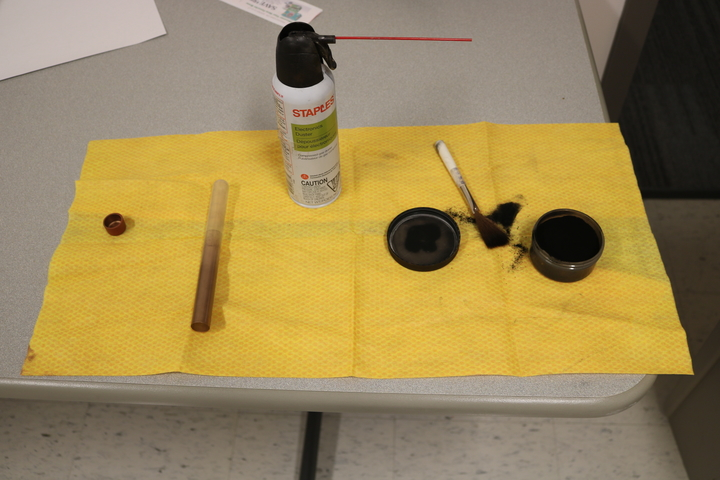
\includegraphics[scale=0.3]{Powder_Stuff}
\caption{Supplies needed for dusting prints}
\label{Figure 1}
\end{figure}

3.	Have the subject sit on the chair, remove a shoe, and loosen the laces.  
4.	Over a trash can, tap the shoe lightly to remove any loose dirt or grass. Some pebbles/dirt that is lodged in the tred is OK and could be a distinguishing characteristic. Under the fume hood and over the plastic container, brush the shoe with print powder. Dip the tip of the brush in the powder and tap the excess off on the side. Carefully, coat the entire shoe out sole in the powder being sure to include all indents, gashes, and grooves (Figure 2). 

\begin{figure}[!htp]
\centering
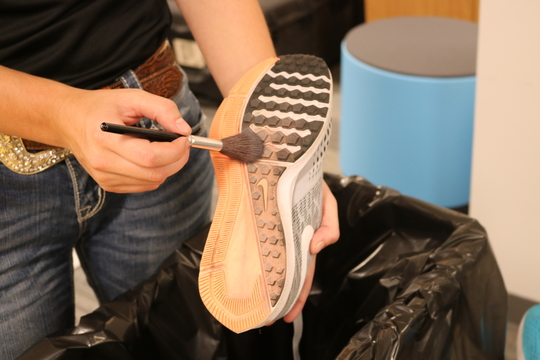
\includegraphics[scale=0.4]{Powder_Brush}
\caption{Coating the shoe with powder.}
\label{Figure 2}
\end{figure}

\newpage

5. Once the shoe is coated, take the hose of the air compressor and blow off any extra powder, still under the hood. Be sure to hold the tip a fair distance from the shoe at an angle as to not blow off all of the powder (Figure 3). 

\begin{figure}[!htp]
\centering
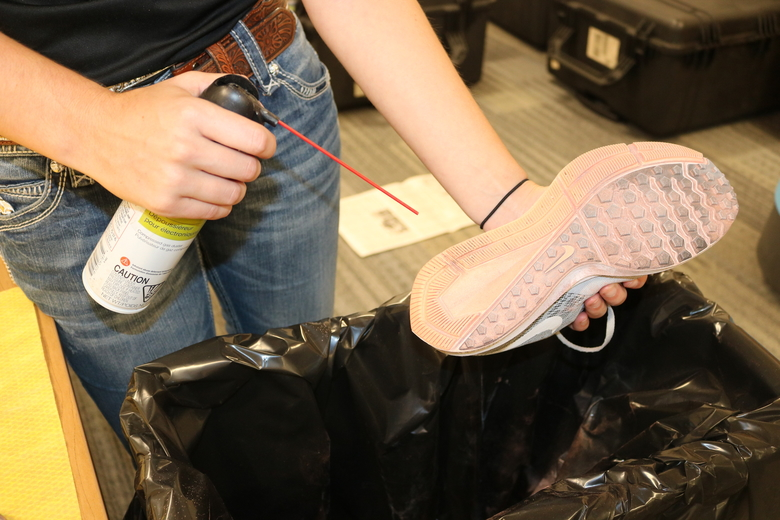
\includegraphics[scale=0.3]{Powder_Air}
\caption{Blowing off any excess powder.}
\label{Figure 3}
\end{figure}

6. Return the shoe to the subject and have them put it on. Be sure that nobody touches the sole of the shoe or brushes off any of the powder. 

7. While wearing a pair of disposable gloves, take a new adhesive film sheet and remove the back. Place it aside for later use. 

8. Place the clear portion, sticky side facing up, in the outline on the news paper. 

9. Guide the subjects shoe down onto the film. The subject should place their heel on the film with their toe pointing towards the ceiling. They will then roll their foot into a flat standing position and step up so that all of their weight is on the film (Figures 4-5). 

\begin{figure}[!htp]
\centering
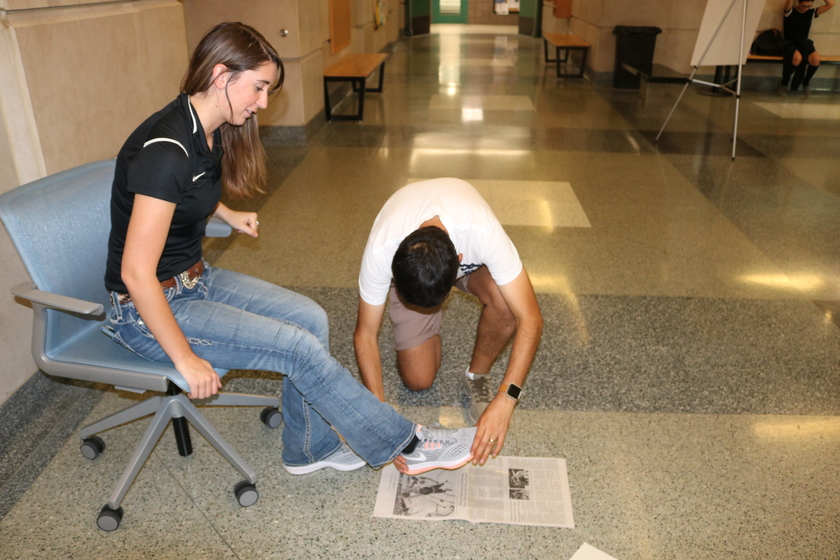
\includegraphics[scale=0.3]{Film_Full}
\caption{Guiding the Subjects shoe down to the film.}
\label{Figure 4}
\end{figure}

\begin{figure}[!htp]
\centering
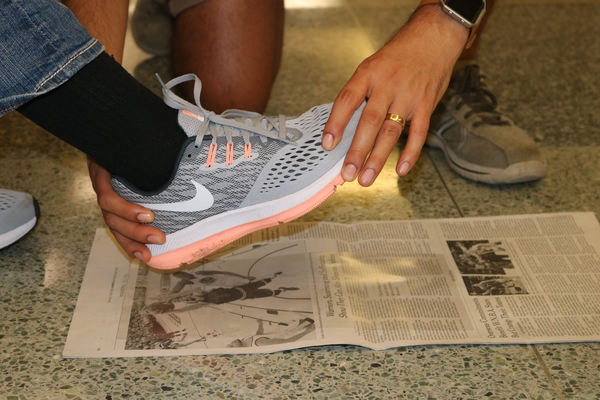
\includegraphics[scale=0.4]{Film_Place}
\caption{First have the heel make contact.}
\label{Figure 5}
\end{figure}

10. The researcher will then place one hand on the front portion of the shoe and use the other to hold the back corners of the film. Carefully, have the subject step off of the film while the hand on the front of the shoe is still keeping light pressure. Peel the foot forward until only the tip of the toe is making contact with the adhesive (Figure 6). At this point, step straight off, but do not place the powdered shoe on the ground. 

\begin{figure}[!htp]
\centering
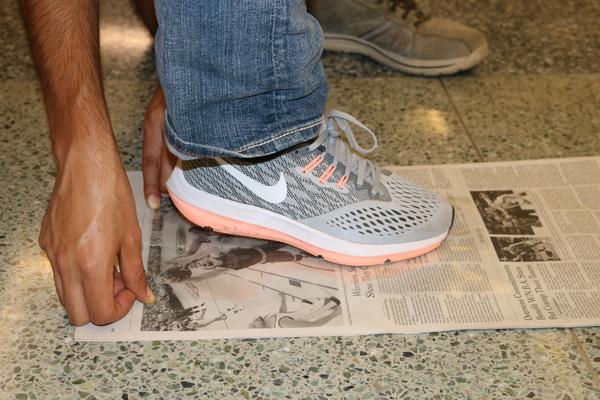
\includegraphics[scale=0.4]{Film_Lift}
\caption{Have the subject step off of the scanner.}
\label{Figure 6}
\end{figure}

11. Have the subject sit back in the chair while keeping the shoe off of the ground. Carefully, place the back onto the film using a roller (Figures 7-8). Please refer to the back of the manual cover page for specific naming procedures and examples.Use the naming tool created by IT to generate the file name. Use the label maker and place a label on the upper right hand corner of the back of the print. Staple the second label to the corner making sure not to damage the print. 

\begin{figure}[!htp]
\centering
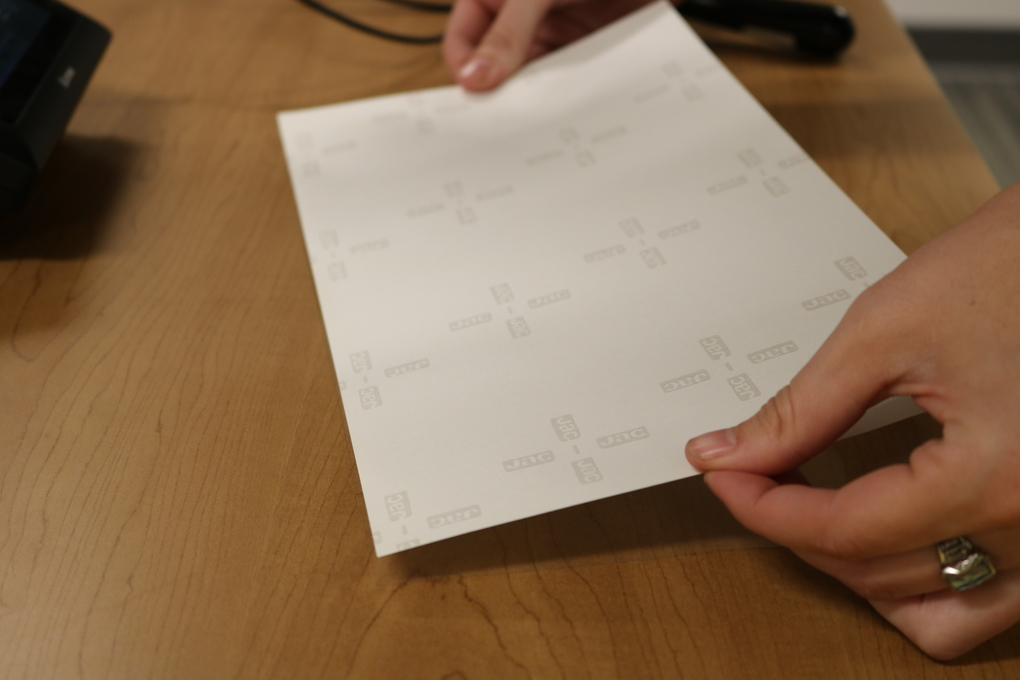
\includegraphics[scale=0.25]{Film_Back}
\caption{Be sure to match up the side and attempt to have no air bubbles.}
\label{Figure 7}
\end{figure}

\begin{figure}[!htp]
\centering
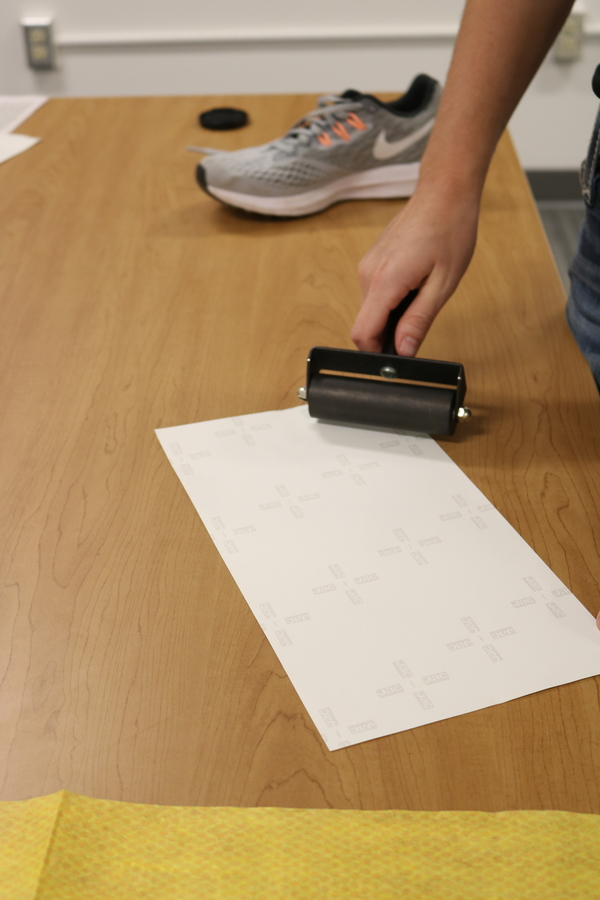
\includegraphics[scale=0.3]{Film_Roller}
\caption{Carefully roll the back of the print to eliminate air bubbles.}
\label{Figure 8}
\end{figure}

\newpage

12. For the second print,take a new adhesive film sheet and remove the back. Place it aside for later use. 

13. Place the clear portion, sticky side facing up, on the news paper near the subject.

14. Guide the subjects shoe down onto the paper. The subject should place their heel on the film with their toe pointing towards the ceiling. They will then roll their foot into a flat standing position and step up so that all of their weight is on the film. 

15. Have the subject lift their foot, with the film attached, so that the sole is facing the tech.Make sure that they at no time shift their foot on the film! At this point, the tech will grab a corner of the film and quickly peel it off. The subject is now free to walk on the shoe. 

16. Carefully, place the back onto the film using a roller. Label the back of the print using the same method as before. File the prints in the correct folder for the cohort for later scanning.

****COMPLEATE REPLICATES FOR SELECTED SHOE PAIRS! SEE LIST IN THE FIRST SECTION OF THIS MANUAL!****

Note: For Film Print scanning, Please refer to the bed scanner procedure. 



\end{document}

